%!TEX root = main.tex
\section{Dataset}
På de følgende sider vil vi gennnemgå vores dataset. Vi vil vise de basale statistikker over dataet og gennemgå afvigelser. Vi vil også gennemgå hvordan vi forholder os til disse afvigelser og hvordan vi lavede datacleaning. \\

Vores data stammer fra Sony's Lifelog\cite{sonyLifeLog} som navnet antyder, er en mobil Lifelog app som logger ens aktiviteter i løbet af dagen. Heri logger den bla. aktivitet i apps og geolokation. Vores dataset stammer fra denne app, indsamlet fra 1586 Sony medarbejdere over 3 måneder\footnote{September 2015 - November 2015} fordelt på 80 lande. 

Vi kan dele datasettet op i 2 dele for oveblikkets skyld: En \textbf{geolokation del} og en \textbf{app og homophily del}. \\


\textbf{Geolokation del}\\
I denne del ligger det mest interessante i forhold til vores problemstilling. Dette er geolokationen for brugeren på et pågældende tidspunkt. Lokationen bliver logget når lokationen ændre sig (værdierne for latitude eller longitude ændre sig). Når lokationen bliver logget, bliver et time stamp også logget (\texttt{start\_time}) - og når lokationen ændre sig, bliver et andet time stamp logget (\texttt{end\_time}). Dvs. at \texttt{start\_time} og \texttt{end\_time} er ens, så længe brugeren er i bevægelse.

Accuracy af GPS og altitude bliver også logget, samt meta-data for pågældende lokation - city name, country, region and area. Table \ref{tab:stat_geo} viser disse attributter samt nogle nøgle værdier. 

\begin{table}[htbp]
        \centering
        \small
        \setlength\tabcolsep{2pt}
        \begin{tabular}{|c|c|c|c|c|c|c|c|c|c|c|}
            \hline
                         & Latitude/  &   start             & end               & Accuracy           & Altitude    & Name   & Country & Region             & Area          \\[-3pt]% compensate for extrarowheight
                         & longitude  &  time               & time              &  (mm)              & (mm)        & (city) &         & (Europe, Asia...)  & (Area/state)  \\
            \hline
                 Unique  &            &                     &                   &                    &             & 19.344 & 80      &                    &               \\
                 entries &            &                     &                   &                    &             &        &         &                    &               \\
            \hline
                 Min     &            &   2015-08-09        &                   &  -2.147.483.500    & -5.086.000  &        &         &                    &               \\
                         &            &   22:25:33.766+02   &                   &                    &             &        &         &                    &               \\
            \hline
                 Max     &            &                     &   2015-12-01      &  500.000           & 17.211.698  &        &         &                    &               \\
                         &            &                     &  01:00:22.711+01  &                    &             &        &         &                    &               \\
            \hline
                 Mean    &            &                     &                   & 35.249             & 105.030     &        &         &                    &               \\
                         &            &                     &                   &                    &             &        &         &                    &               \\
            \hline
                 Std.    &            &                     &                   & 3.672.390          & 403.966     &        &         &                    &               \\
                 dev.    &            &                     &                   &                    &             &        &         &                    &               \\
            \hline
        \end{tabular}
        \caption{Overview and statistic summary of geolocation dataset} %add this between 'caption' and '{...' for new text in listing of tables: [New caption text only for listing of tables]
        \label{tab:stat_geo}
\end{table}

Distributioner

\begin{figure}[H]
    \centering
    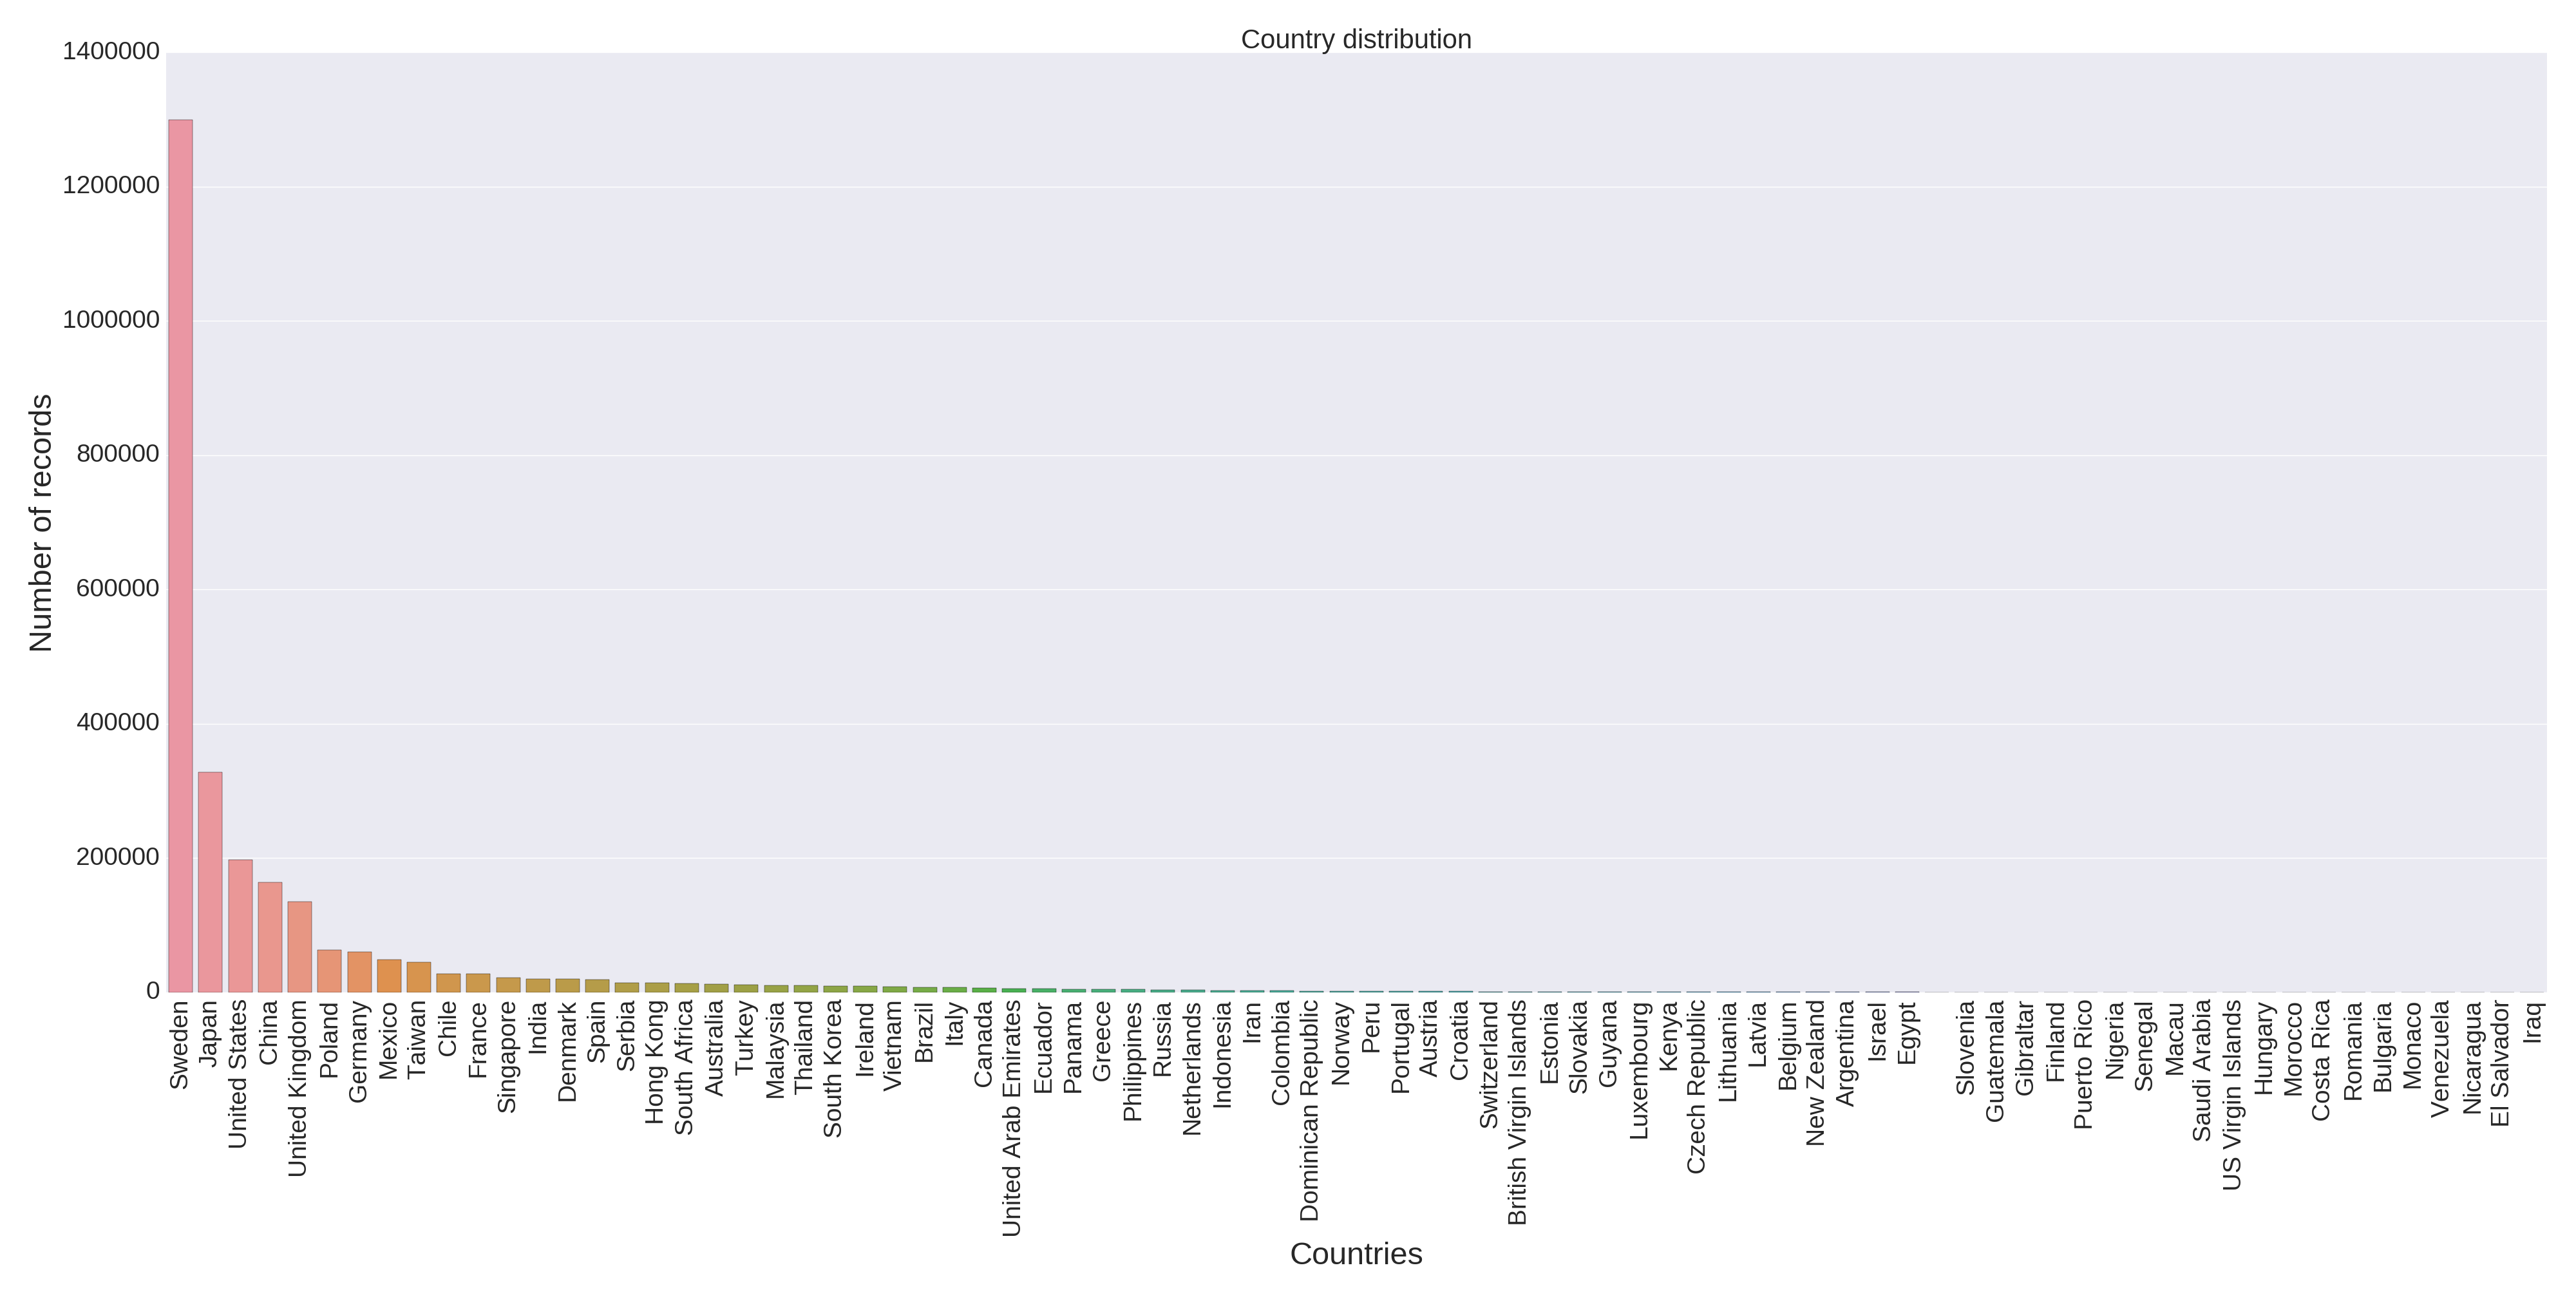
\includegraphics[scale=0.18]{country_distribution}
    \caption{Awesome Image}
    \label{fig:awesome_image}
\end{figure}
Outliers



Som man kan er der lidt færrer lande end det vi tidligere skyldtes. Dette 

Our work will focus on the location updates from Japan. There is 332 users in Japan for which we have location updates.
When training our classifier we divided the dataset into three parts where each corresponded to a month.

Japan locations for September: 340198
Japan locations for October: 208242
Japan locations for November: 102442

\textbf{App og homophily del}\\


Over disse 3 måneder blev der indsamlet 2.665.893 geolokation records, som er vores primær data. 
\textcolor{red}{When we got the dataset it was divided into multiple Apache Avro files which is a data serialization framework for Hadoop.\cite{apacheavro}}

